\subsection{Learning End-to-End Goal-Oriented Dialog \cite{Bordes2016Learning}}

The main contributions of the paper are: (1) propose to evaluate end-to-end dialogue systems using goal-oriented tasks, and design five tasks in the application of restaurant reservation; (2) apply Memory Networks to train an end-to-end dialogue system, and show that per-response performance is encouraging.

The five tasks are (1) issue API calls. The system should ask questions, gather information about the preferred cuisine type, location, price range, and party size of restaurants, and generate the correct API call; (2) update API calls. When user preferences change, the system should update the API call; (3) display options. The system should propose the restaurants, which match user preferences, until users accept; (4) provide extra information. When users ask for the phone numbers and address of a restaurant, the system should answer correctly based on the facts; (5) conduct full dialogues (see Figure \ref{fig:Bordes2016Learning01} for examples of the five tasks). Natural language patterns and knowledge base entities are combined to generate simulated dialogues consisting of user and system utterances.

\begin{figure}[htbp]
  \centering
  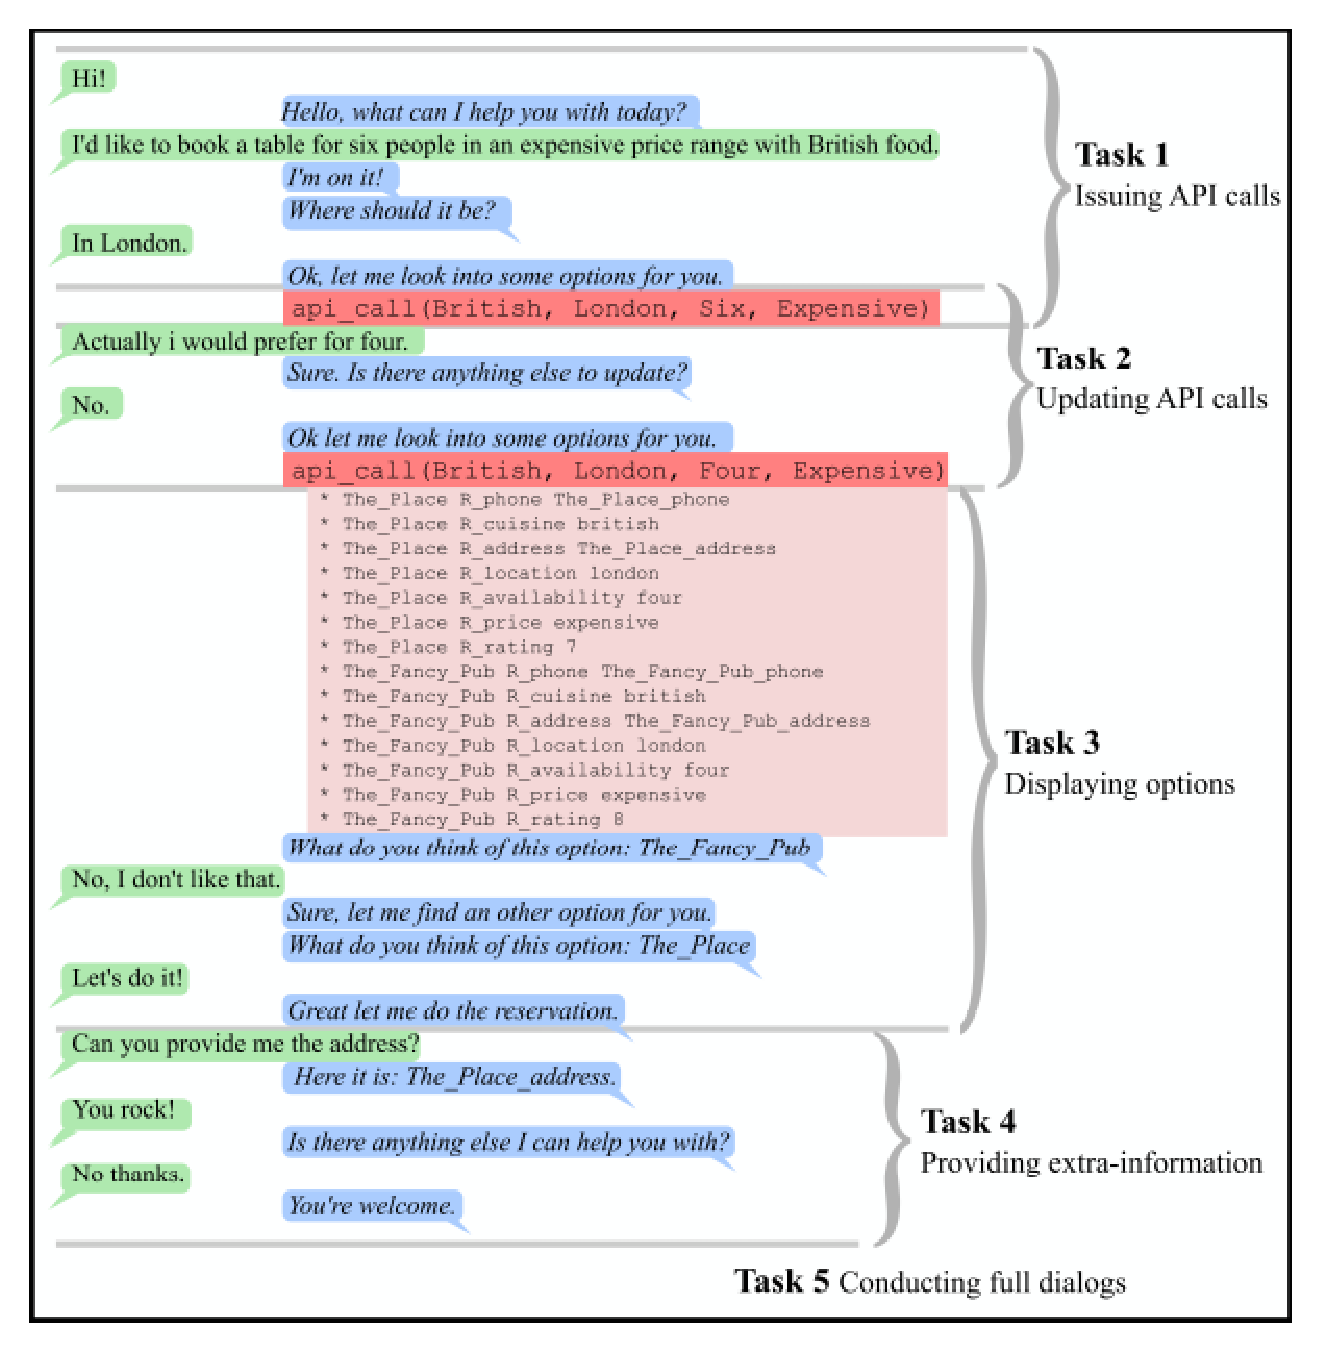
\includegraphics[width=.8\linewidth]{Bordes2016Learning01}\\
  \caption{Examples of the five tasks}\label{fig:Bordes2016Learning01}
\end{figure}

The paper uses a retrieval-based method, i.e. selecting the best candidate response from a large set of all possible system utterances and API calls. The paper applies Memory Networks that consist of three component (1) store conversation in memory; (2) read pertinent information from the memory; (3) use the information to output the best candidate response. 